% HA Schema


\chapter{High availability schema}
\label{chap:ha-schema}
This chapter explains the High Availability system that will be tested through the Thesis. 

\section {Main schema}
There are two servers which we will name the primary one and the secondary one. Each of them are linked by two means. The service link is the main network interface which it's connected via a normal switch. It will serve content to the final users. The communication link, which it's used for the cluster management and syncronisation is done via a crossover cable.

We can see the main schema, where we have added two final clients at figure \ref{fig:main-schema}.

\begin{figure}
  \centering
    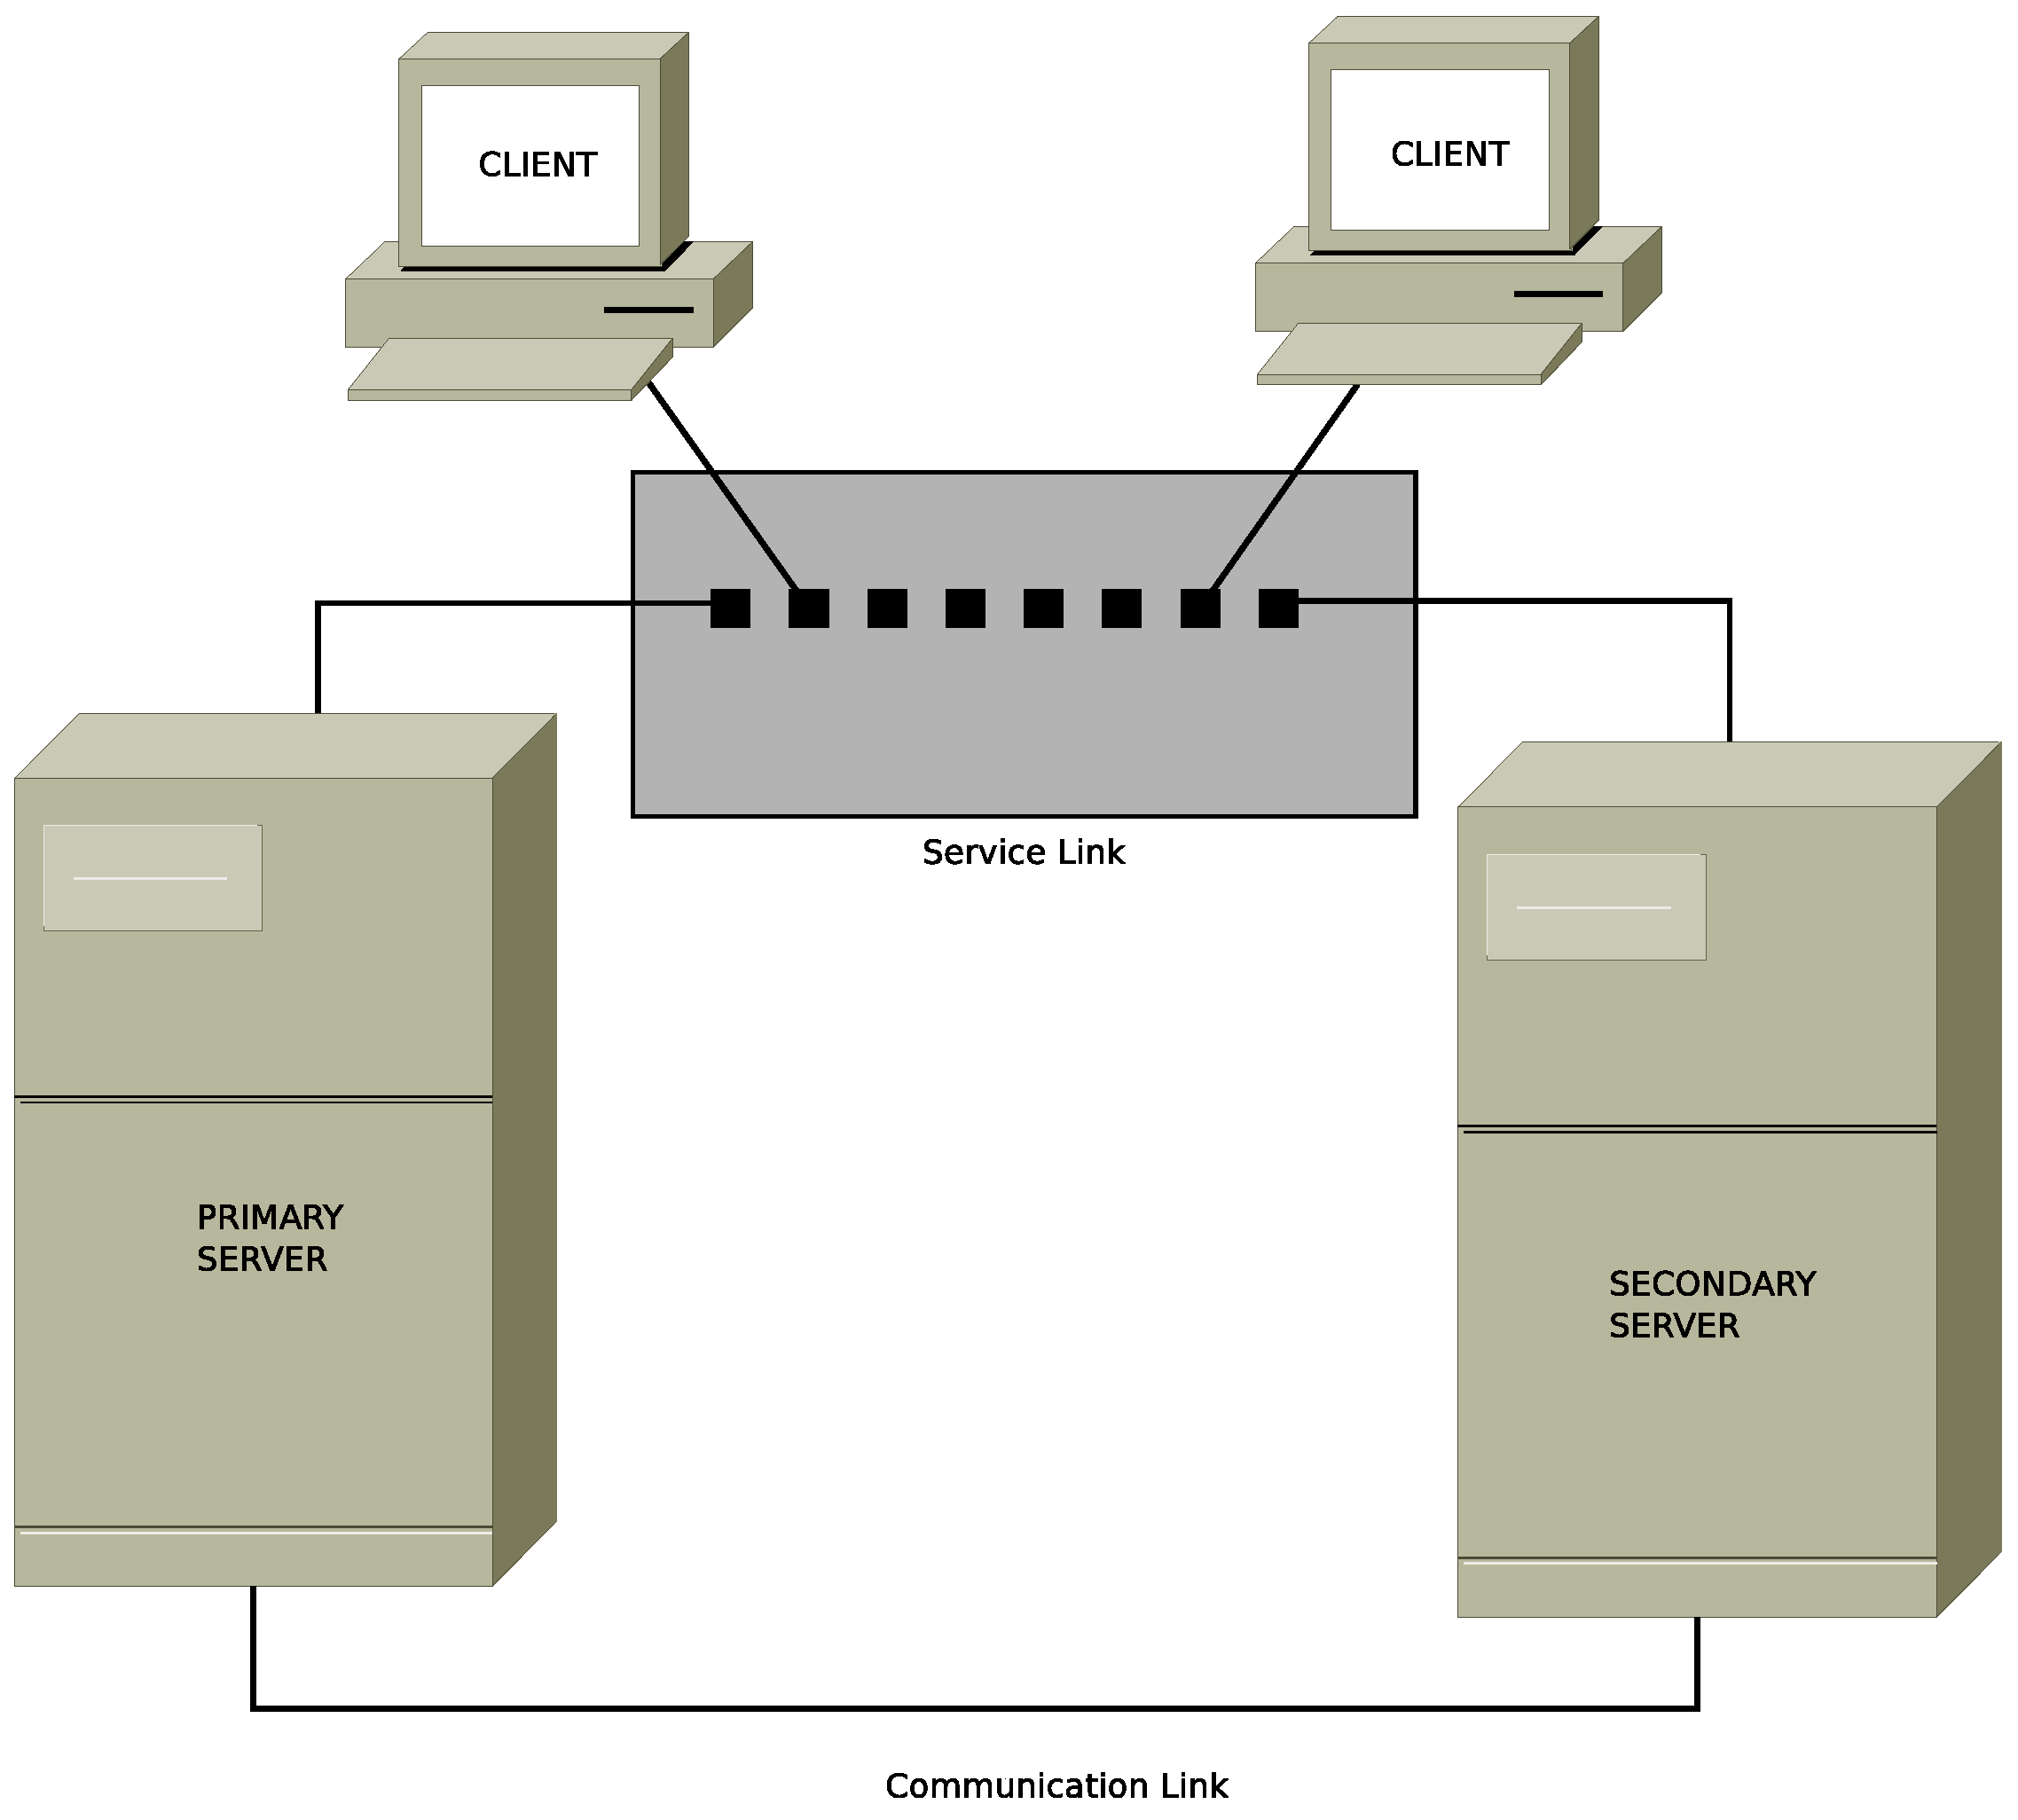
\includegraphics[width=0.8\textwidth]{img/ha_main_schema.eps}
  \caption{High Availability main schema}
  \label{fig:main-schema}
\end{figure}

\section {Primary server}
\subsection {Specifications}
The primary server specifications are as follow:
\begin{itemize}
  \item RAM: 4 GB
  \item Hard disk: 100 GB
  \item Processor: 2 x 2,40 Ghz
\end{itemize}

\section {Secondary server}
\subsection {Specifications}
The primary server specifications are as follow:
\begin{itemize}
  \item RAM: 4 GB
  \item Hard disk: 100 GB
  \item Processor: 2 x 2,40 Ghz
\end{itemize}

\section {Virtualbox implementation}
\subsection {Introduction}
Although in production environments High Availability systems are implemented in Physical servers or highly optimised virtualised servers we are going to use Oracle VM Virtualbox software to simulate the described system. This section summaries how to create both virtual machines and link them.

\subsection {\label{subsec:primary-virtual-machine-creation}Primary Virtual Machine creation}
We click on \textit{Machine} menu and select \textit{New} option. The Create Virtual Machine wizard will appear.

\subsubsection {Name and operating system}
\begin{itemize}
  \item Name: PrimaryZimbraHA
  \item Type: Linux
  \item Ubuntu (64 bit)
\end{itemize}

\subsubsection {Memory size}
Zimbra needs: 2048 MB as a minimum.
\subsubsection {Hard drive}
We select \textit{Create a virtual hard drive now}, \textit{Virtualbox Disk Image} as the hard drive file type, Dynamically allocated (so that the hard drive file only uses space as it fills up).

We leave the default File location and select hard disk size as 110 GB which it's quite bigger than the strictly needed for our high availability system.

\subsection {\label{subsec:service-link-primary}Service link network on Primary Virtual Machine}
We select \textit{PrimaryZimbraHA} virtual machine and click on \textit{Machine} menu and then in \textit{Settings} option. We will make sure we are in \textit{Network} section.

We will use default \textit{Adapter 1} for service link. We are going to summarise its setup:
\begin{itemize}
  \item Attached to: \textit{Internal Network}
  \item Name: ZimbraHAService
\end{itemize}

Finally we click on OK for saving changes.

\subsubsection {Secondary Virtual Machine creation}
In order to create secondary virtual machine we can either repeat the same steps as in \textbf{\ref{subsec:primary-virtual-machine-creation} Primary Virtual Machine creation}. Or we can make a linked clonation of the original machine. We will describe the latter option.

We select PrimaryZimbraHA virtual machine and then in \textit{Machine} menu we select \textit{Clone} option.

\textbf{New machine name}
\begin{itemize}
  \item New machine name: SecondaryZimbraHA
  \item Reinitialize the MAC address of all network cards: Checked
\end{itemize}

We select \textit{Linked clone} as Clone type.

Finally we click on \textit{Clone} button so that cloning is performed.

\subsection {Service link network on Secondary Virtual Machine}
As we did in subsection \textbf{\ref{subsec:service-link-primary} Service link network on Primary Virtual Machine} we select \textit{SecondaryZimbraHA} virtual machine and click on \textit{Machine} menu and then in \textit{Settings} option. We will make sure we are in \textit{Network} section.

We will use default \textit{Adapter 1} for service link. We are going to summarise its setup:
\begin{itemize}
  \item Attached to: \textit{Internal Network}
  \item Name: \textit{ZimbraHAService}
\end{itemize}

If we have cloned the virtual machine settings might be correct by default.

Finally we click on OK for saving changes.

\subsection {Communication link}
For both PrimaryZimbraHA and SecondaryZimbraHA virtual machines we will perform a very similar operation than the one done in subsection \textbf{\ref{subsec:service-link-primary} Service link network on Primary Virtual Machine}.

But now we make sure that we \textit{Adapter 2} is enabled as an \textit{Internal Network} which name is \textit{ZimbraHACommunication}.

\subsection {NAT link}
In order to make installation easier we will enable \textit{Adapter 3} in both virtual machines so that it can use the host Internet in order to fetch packages and perform post installation setup.

Similarly to subsection \textbf{\ref{subsec:service-link-primary} Service link network on Primary Virtual Machine} we make sure that \textit{Adapter 3} is enabled and that it's attached to NAT.

\subsection {Email client Virtual Machine}
A Virtual Machine whose only purpose is to test high availability from a service link point of view might be added if needed. We're not to cover the installation and its setup here. We will just mention its network setup is similar to PrimaryZimbraHA and SecondaryZimbraHA but removing the second interface which serves for communication link and that, of course, doesn't make sense in an Email client VM.